\documentclass[12pt]{article}

\usepackage[margin=1.0in]{geometry}
\usepackage{graphicx}
\usepackage{listings}
\usepackage{tabto}
\usepackage{multicol}
\usepackage{lipsum}
\usepackage{caption}
\usepackage{mwe}
\usepackage{tikz}
\usepackage{tabto}
\usetikzlibrary{automata,positioning}
\usepackage{enumitem}
\usepackage{amsmath}
\usepackage{amssymb}
\graphicspath{ {./} }

\begin{document}

\title{CS4337 : Database Systems\\Quiz 4, 5, 6, 7, 8 }
\author{Matthew McMillian\\mgm160130@utdallas.edu}
\maketitle


\begin{enumerate}
	
	\item a) The relation is in 1st normal form. We have a transitive relationship, however some of the 'Y' functional dependencies are not dependent on the 'X' values (as in 'X $\rightarrow$ 'Y'). \\
b) There is no need to normalize this any further

	\item Doctor Number, Patient Number, Date $\rightarrow$ Diagnosis\\
Diagnosis $\rightarrow$ Treat$\_$code\\
Treat$\_$code $\rightarrow$ Charge\\

This relation is in 2nd normal form since all non-key elements are dependent on the table's primary key(s), since the Patient number depends on which doctor
they have, and the diagnosis of the patient depends on what the patient has. The charge and Treat code are dependent on the diagnosis. This is not in 3rd
normal form since a nonkey attribute is defined by another nonkey attribute (Treat$\_$code $\rightarrow$ Charge).

	\item ACID properties include Atomicity, Consistency, Isolation, and Durability. Atomicity says that a operation (transaction) must occur completely, or not at all,
meaning we cannot have any partial transictions to prevent data corruption. Consistency states that any crud operation is consistient with the rules of the
database, that is, a crud operation cannot violate the database conditions. Isolation is another form of mutual exclusion, that is, transactions cannot interfere
with eachother otherwise data may get corrupted. Durability means that transactions will persist in the database, that is, a transaction will remain committed
(not partially committed) even if a database fails. If a transaction commit fails mid commit, the commit will not fully go through to preserve the data.

	\item A query tree represents a relation algebra expression. Similar to a parse tree in automata theory, it breaks down an expression and executes the desired query.
The query trees primary purpose (following database rules) attempts to execute the most efficient queries (least amount of operations, calls, joins, etc.)

	\item 2 phase locking is a deadlock prevention measure that attempts a no-preemption strategy, that is, no process is ever in a state where it is holding shared resources.
There are two parts to this strategy, the growing and shrinking phase. The growing phase allows new locks to be put on data items but does not allow for locks to be replaced.
The shrinking phase allows for existing locks to be released by for no new locks to be acquired. This makes sure that if a process is gaining or releasing their locks,
that no other process can access it until all their resources are given up.

	\item (512+128)*20 = 12800bytes $\rightarrow$ Total Capacity\\
(512)*20 = 10240bytes $\rightarrow$ Useful Capacity\\
Cylinders = 400 (same as tracks)\\
(512+128)*20*30 = 384000bytes $\rightarrow$ Total Capacity of a cylinder\\
(512)*20*30 = 307200bytes $\rightarrow$ Useful Capacity of a cylinder\\
(512+128)*20*30*400 = 153600000bytes $\rightarrow$ Total Capacity of a disk pack\\
(512)*20*30*400 = 122880000bytes $\rightarrow$ Useful Capacity of a disk pack\\
transfer rate = track capacity / rpm*60*1000 $\rightarrow$ 12800 / 2400*60*1000 = 88.9 bytes a second\\
block transfer time = blocks/tr = 512/88.9 = 5.76 millsec\\
rot delay = 1/2(1/2400)*60*1000 = 12.5 millsec\\
average seek time is blocktrans + rot del + seek time = 5.76 + 12.5 + 30 = 48.26 millisec\\
20 random blocks = blocks*(seek + rot + block trans) = (48.26 millisec) * 20 = 965.2 millisec\\
20 consecutive w/ bufffer = (seek + rot + blocks*block trans) = 157.7 millisec\\
	
	\item record = name + ssn + deptcode + addr + phone + bdate + sex + jobcode + sal = 30 + 9 + 9 + 40 + 9 + 8 + 1 + 4 + 4 + 1 = 115 bytes per record\\
blocking factor = average record per block = 115 / 512 = 4.45, or about 4 records per block\\
number of blocks = 30000/4 approx 7500\\
index blocks = index block size + key size = 6 + 9 = 15 bytes\\
index block factor = blocks / index block = 512/15 = 34\\
7500 entries in block, 7500 first level keys\\
number of first-index-blocks = 7500/34 = 221 blocks\\
number of 2nd-level index entries = number first level blocks = 221\\
number of 2nd level blocks = ceil(2nd level entries/1st block factor) = 221/34 = 7\\
number of 3rd-level index entries = 7\\
number of 2nd-level index = ceil(blocks/block factor) = ceil(7/34) = 1 $\rightarrow$ we have 3 levels\\
total number of blocks = 221 + 7 + 1 = 229\\
number of block accesses = x + 3 = 1 + 3 = 4\\

	\item student:\\
sname, snum, sssn, scaddr, scphone, apaddr, spphone, bdate, sex, class, majordeptdcode, minordeptcode, prog\\

dept:\\
deptname, deptcode, deptoffice, deptphhone, deptcollege\\

course:\\
cname, cdesc, cnum, cdept,\\

section:\\
instructorname, semester, year, seccourse, sectionnum\\

grade:\\
ssn, grade\\

relations:\\
deptcode$\rightarrow$ majordeptcode, minordeptcode, cdept\\
seccourse $\rightarrow$ course\\
ssn $\rightarrow$ sectionnum\\

functional dependencies:\\
snum, sssn $\rightarrow$ sname, scaddr, scphone, apaddr, spphone, bdate, sex, class, majordeptdcode, minordeptcode, prog\\
deptname, deptcode $\rightarrow$ deptoffice, deptphhone, deptcollege\\
cnum $\rightarrow$ cname, cdesc, cdept\\
sectionnum, seccourse, year, semester $\rightarrow$ instructor\\
sectionnum, seccourse, year, semester, ssn $\rightarrow$ grade\\

This relation is not in 3rd normal form since not all non-primary key attributes are dependent on the primary key. I.e. snum and sssn. This is in 2nd normal form.

	\item Where (a) and (b) with m=2 and n=2 could be problematic. If the value of x is greater than 90 (since the addition and subtraction of m and n cancel out),
then we have a missing commit issue since the thread will exit before writing X. There is not really a change, since even though we are not writing the
added value back, we are writing it back before the if statement is called, making our addition useless.

	\item No, in this case it would not make a difference. Since A has not been written yet, only read, the rollback process doesn't not need to change.
	
	\item A deferred update strategy doesn't log and write operations until the transaction commits. The log would change since all the write transactions would come after
the commits, as seen below:\\

start$\_$transaction T1\\
read$\_$item T1 A\\
read$\_$item T1 D\\
commit T1\\
write$\_$item t1 D 20 25\\
checkpoint\\
start$\_$transaction T2\\
read$\_$item T2 B\\
start$\_$transaction T4\\
read-item T4 D\\
start$\_$transaction T3\\
read$\_$item T4 A\\
commit T4\\
write$\_$item T4 D 25 15\\
write$\_$item T4 A 30 20\\
read$\_$item T2 D\\

however, the following operations are ignored...\\
write$\_$item T2 D 15 25\\
write$\_$item T3 C 30 40\\
write$\_$item T2 B 12 18

	\item A table scan iterates over all the rows of a table instead of using some indexed table. An example is if you are trying to do a SELECT (elements) from a table,
instead of selecting indexes from a page table and getting their exact location the table scan will go through the entire table.

	\item Table scans are undesirable because they do unneeded work. That is, they have a large time complexity (linear).
	
	\item Table scans can be avoided by using a page table, or some other indexing strategy for direct lookup rather than scanning through the entire table.
	
	\item a.) A schema defines relations\\
b.) A relation has attributes\\
c.) A relation applies to groups of tuples
 	
 	\item  SELECT PNO\\
  \tabto{1cm}FROM ((WORKS$\_$ON) JOIN (SELECT Ssn FROM ( SELECT *\\
                           \tabto{2cm}FROM EMPLOYEE E WHERE E.Lname = 'Smith' )))\\
                           \tabto{2cm}UNION\\
                           \tabto{2cm}(SELECT PNO\\
                             \tabto{3cm} FROM ((SELECT Dnumber (SELECT *\\
                                       \tabto{3cm}FROM (SELECT Lname, Dnumber\\
                                         \tabto{4cm}      FROM EMPLOYEE E)\\
                                              \tabto{4cm}WHERE Lname = 'Smith')))\\
                                             \tabto{4cm} JOIN (SELECT *\\
                                                 \tabto{3cm}     FROM DEPARTMENT\\
                                                 \tabto{3cm}    WHERE Ssn=Mgr$\_$ssn))\\
                                                 \tabto{3cm}   JOIN (SELECT *\\
                                                  \tabto{2cm}         FROM PROJECT\\
                                                     \tabto{1cm}       WHERE Dnumber=Dnum)\\

	\item DML
	
	\item DDL is the data definition language used to define tables, and other structural elements of the database
	
	\item You authorize a user by calling the GRANT keyword, followed by the user and the list of privileges you wish to give them. To create a user
you call CREATE USER [username] IDENTIFIED BY [password].

	\item One way to remove duplicate elements from SELECT's result set is to apply the distinct keyword, which will return only unique rows from the result set.

	\item D, the commit operation. When you make a change to the database it does not fully 'change' the database until you execute a commit command.

	\item c. Foreign key to Primary Key
	
	\item A. Group By. When doing aggregate functions, you need to specify (if you choose to return more than just the aggregate) what subset of data you wish to specify the aggregate function by.
	
	\item D is not necessarily true, therefor it is not true of views
	
	\item The record blocking factor is the amount of records that fit into a block of memory.
	
	\item The query tree will try to derive an optimal tree heuristically in hopes to obtain a parsing pattern. Alternatively dynamic programming can be used when searching for multiple attributes to save processing time when rescanning for another attribute.
	
	\item There are 4 isolation levels, uncommitted read, committed read, repeatable read, and serializable.
Uncommitted read allows for data reading while a commit is taking place. Committed Read states that
a read will never occur while uncommitted changes have been made. Repeatable read states that if a
read operation is issues twice with the same query, that both read operations will return the same value.
Serializable ensures that if a query is issued again, that no data will no new data / rows will appear.
This is mainly used for concurrent operations.

	\item Since 2 phase locking takes a no preemption strategy, this on its own states that processes cannot hold shared resources. If all processes are under this strategy,
it means that no deadlocks can occur, which implies that all transactions can run concurrently. i.e. all their transactions can complete correctly without fear of deadlock.
	
	\item File layout (and file allocation) is typically handled by the Operating System, i.e. these operations are done at a physical database level.
	
	\item Typically to get into 2nd and 3rd normal form, you must go through a normalization process. First, you must convert a table into first normal
form before converting to 2nd or 3rd. Once in 2nd normal form, then you can convert to 3rd normal form, etc. This process continues for each normal
form you convert to.
	
	\item No, it is not true that all functional dependencies are symmetric.  A $\rightarrow$ B does not imply B $\rightarrow$ A, especially in key/nonkey relations.
	
	\item 'an unrepeated data' form
	
	\item Indexing and other optimization help reduce the time needed to search for items in select statements
	
	\item Unspanned records create gaps within blocks. Since you cannot span a record across multiple blocks, you create spaces within the blocks of memory that are unused. This is also known as fragmentation.
	
	\item Unordered data files do not have index tables, which save space
	
	\item The main purpose of using an index is to keep track of where records are stored, and it allows for a faster lookup time (in most cases)
	
	\item A second index could be used in a 2 layered key system to simulate a B-Tree file system. This file structure would allow for log(n) lookups which keeping a linear space, a 'in the middle' strategy comparative to single indexing and unordered files.
	
	\item  The schedule itself is not schedule serializable since all actions of a single transaction do not occur consecutively, however there are no conflicts within the
 schedule so with a little rearranging we can make the schedule serializable.

	\item B. A read lock is considered a shared lock since other transactions are allowed to read the item.
	\pagebreak
	\item The EER Diagram: \\
	\begin{center}
			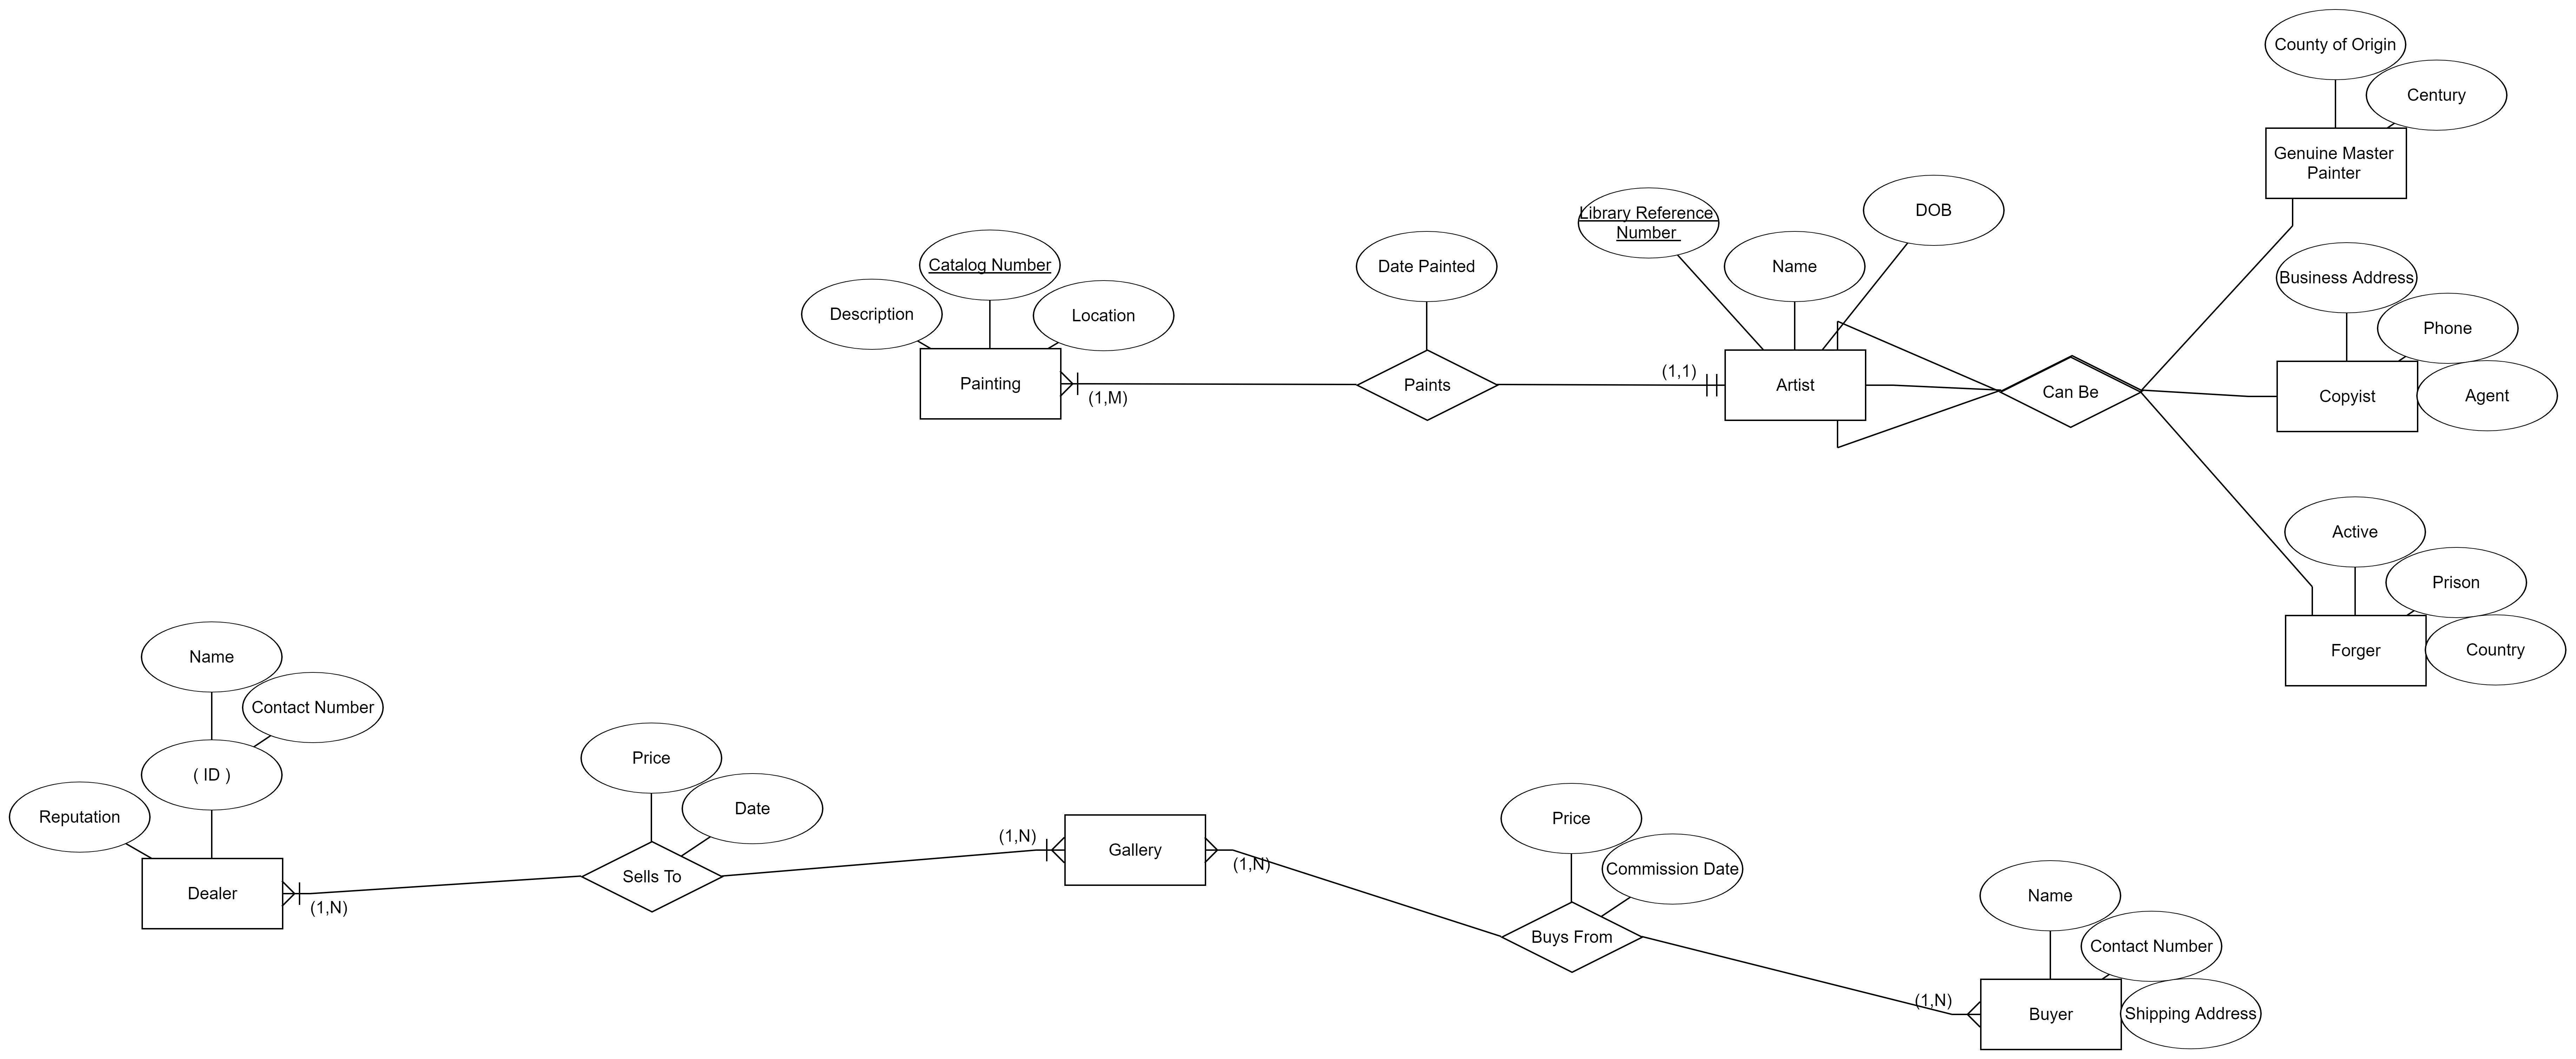
\includegraphics[scale=.06]{40}
	\end{center} 
		
	\item The ER Schema: \\
	\begin{center}
			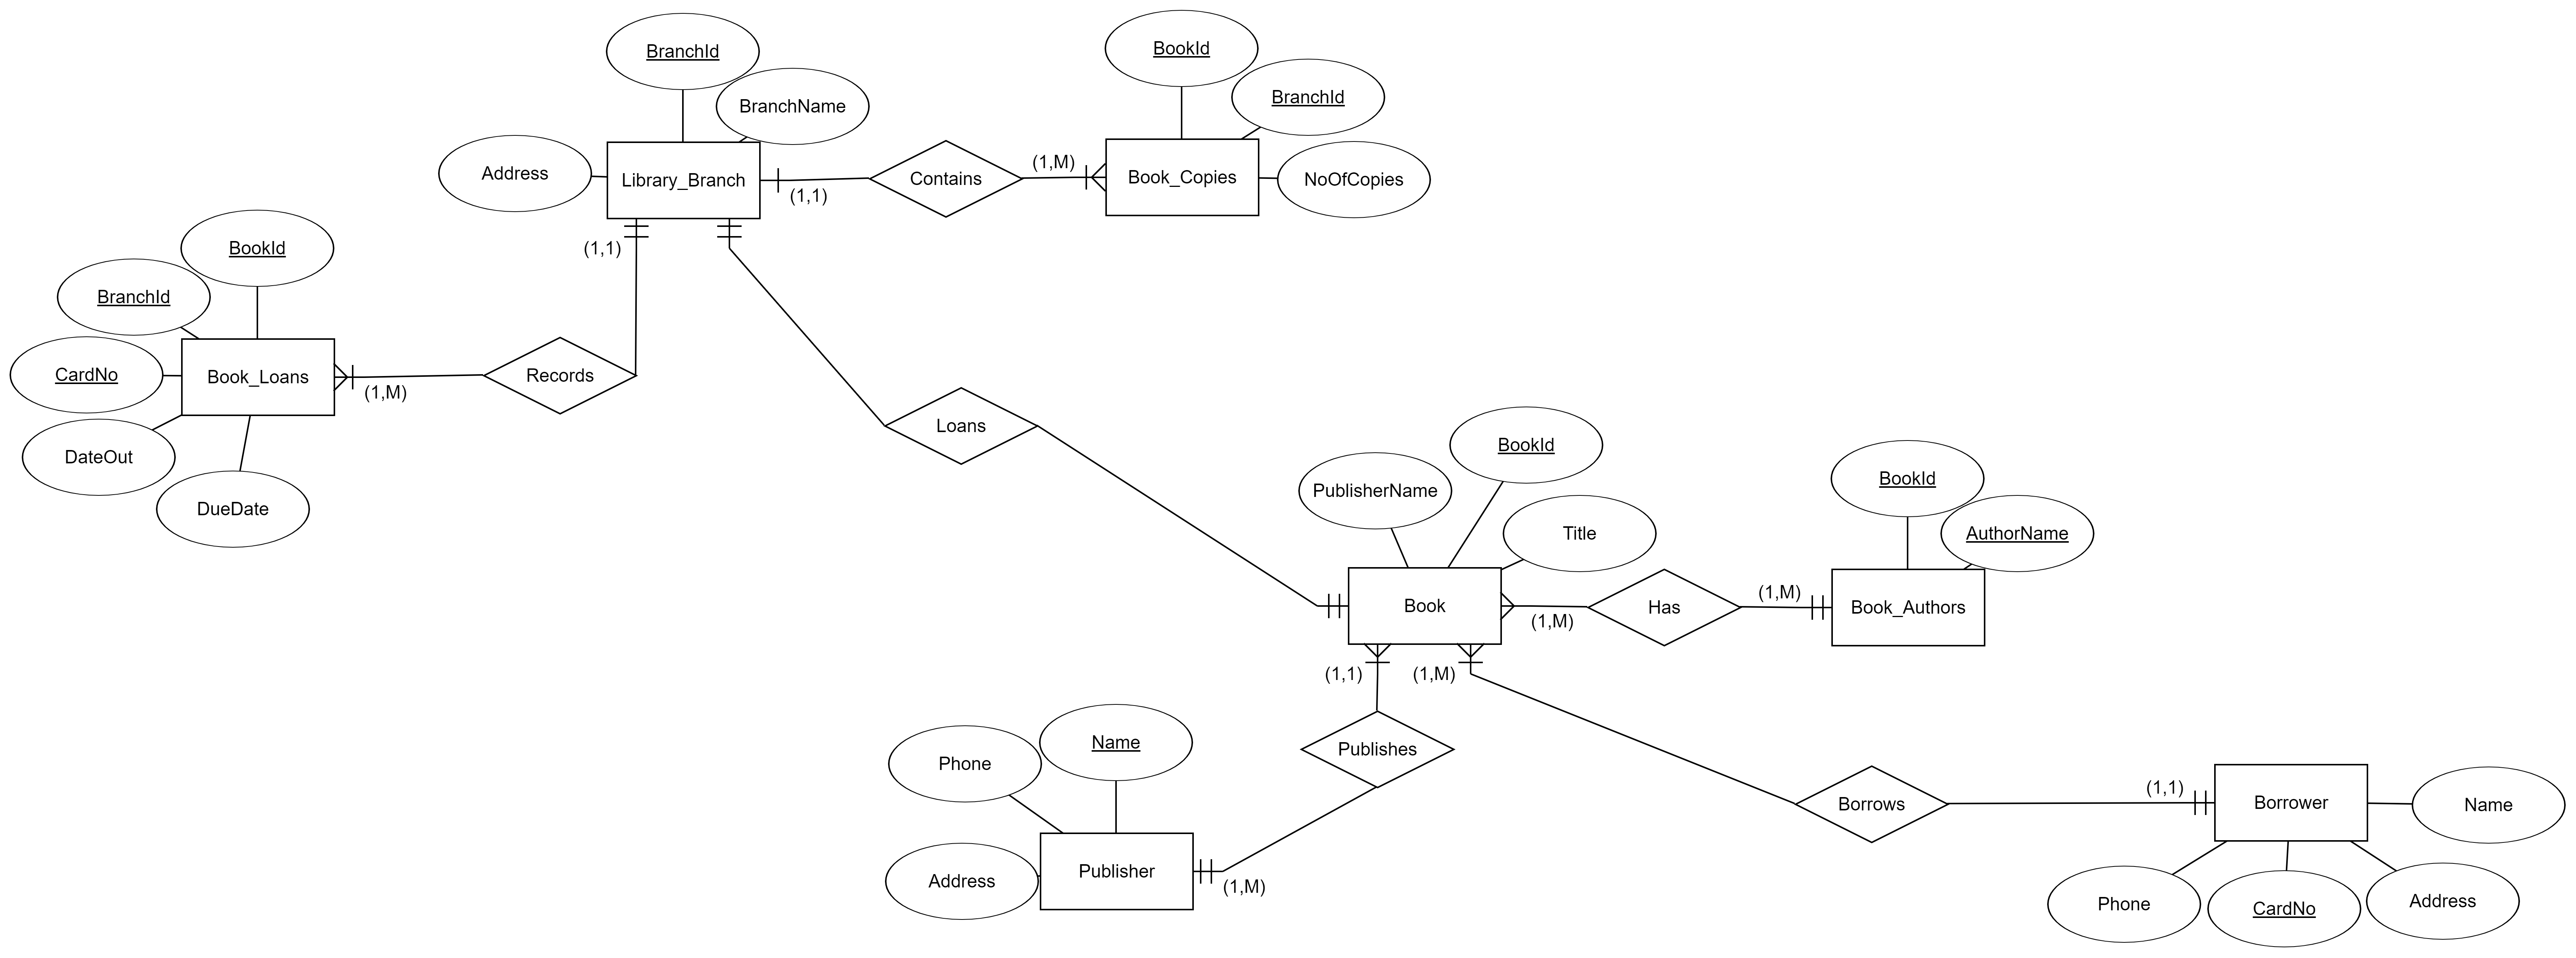
\includegraphics[scale=.07]{41}
	\end{center} 
	
	\item C is wrong, since there is an optional subclass split with no parent class
	
	\pagebreak	
	
	\item The Relational Schema: \\
	\begin{center}
			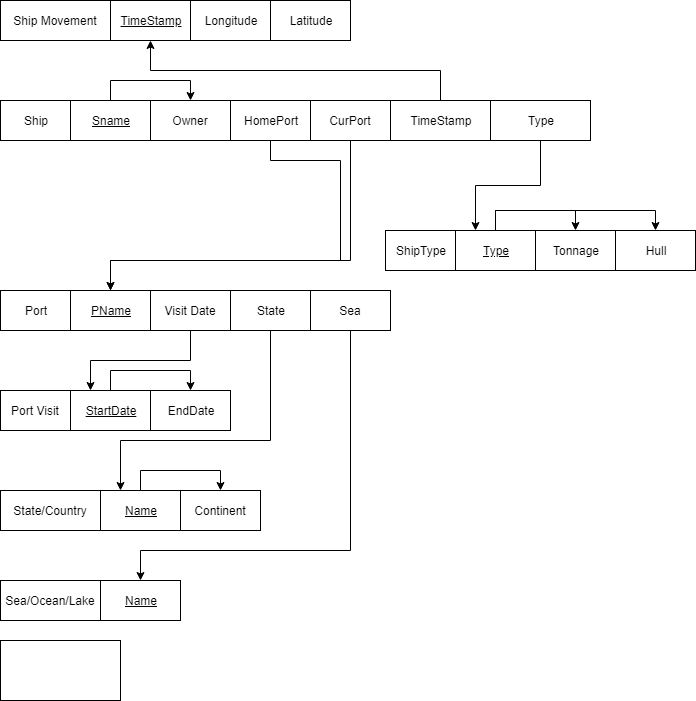
\includegraphics[scale=.5]{43}
	\end{center} 
	
	\item A commit operation makes a database's actions permanent.

\end{enumerate}


\end{document}
